\documentclass[aip,jap,reprint,floatfix,nofootinbib]{revtex4-2}

\usepackage{graphicx}
\usepackage{amsmath}
\usepackage{amssymb}
\usepackage{booktabs}
\usepackage{hyperref}

\begin{document}

\title{Toward Self-Organized Magnonic Crystals in Ferromagnetic\\Shape Memory Alloys}

\author{C.~Scott}
\affiliation{APTSystems.ai, Enumclaw, Washington, USA}

\date{\today}

\begin{abstract}
Magnonic crystals---periodic magnetic structures that control spin wave dispersion---are nearly always lithographically fabricated, which constrains them to two-dimensional thin-film geometries and to a small number of discrete states. We investigate whether martensitic twin variants in ferromagnetic shape memory alloys can function as a self-organized magnonic crystal that requires no lithography. Twin boundaries between crystallographic variants create natural magnetic discontinuities that scatter spin waves, and the variant pattern---whose periodicity is set by thermodynamics rather than patterning---determines the resulting magnonic band structure. Using a linearized Landau-Lifshitz-Gilbert transfer-matrix model, we compute the dispersion relation $\omega(q)$ and transmission spectrum for a one-dimensional Ni-Mn-Ga variant chain. We find structured frequency response with nearly complete transmission suppression in multiple bands, and the transmission fingerprint changes dramatically under simulated magnetic field-driven variant reorientation (Pearson $r$ falling from $1.00$ to approximately zero). We also quantify the effect of positional disorder, finding that the clean periodic band gap broadens into a disorder-tolerant frequency-selective attenuation region. A 2D micromagnetic simulation using mumax3 provides a qualitative consistency check. These results suggest that martensitic variants may offer an alternative route to magnonic crystals that avoids lithographic fabrication and enables continuous reprogramming; experimental validation is proposed.
\end{abstract}

\maketitle

\section{Introduction}
\label{sec:introduction}

Magnonic crystals---the magnetic analogue of photonic crystals---enable engineered control of spin wave dispersion through periodic modulation of magnetic parameters~\cite{Nikitov2015,Chumak2015,Krawczyk2014,Barman2021}. They underpin proposals for spin wave logic gates~\cite{Schneider2008}, magnonic interconnects~\cite{Vogt2014}, and phase-based computing~\cite{Fischer2017}. Recent advances have demonstrated reconfigurable magnonic crystals using current-driven domain wall motion~\cite{Gallardo2022} and stripe domain transitions~\cite{Graczyk2024}.

However, most existing magnonic crystals are lithographically fabricated. Whether patterned as nanodisk arrays~\cite{Ding2021}, ion-implanted waveguides~\cite{Obry2013}, or exchange-biased stripes~\cite{Heussner2020}, their periodicity is defined by e-beam or optical lithography. This constrains them to two-dimensional thin-film geometries, limits scalability, and makes reprogramming between more than a few discrete states difficult. A magnonic crystal that self-assembles and can be continuously reprogrammed would represent a useful alternative.

Although the magnetic shape memory behavior of Ni-Mn-Ga is well characterized~\cite{Heczko2014}, to our knowledge the periodic twin variant lattice has not previously been analyzed as a self-organized magnonic crystal---that is, as a structure whose translational symmetry produces Bloch band structure, frequency gaps, and field-reconfigurable periodicity. This may be because the magnonics community has focused primarily on lithographically defined structures, while the shape memory community has focused on strain and actuation rather than spin wave propagation. The conceptual bridge between these two fields is the contribution of this paper.

Figure~\ref{fig:schematic} illustrates the physical system. A one-dimensional chain of alternating twin variants A and B, with distinct magnetocrystalline easy axes, forms a periodic magnetic structure. Spin waves propagate along the chain and scatter at each twin boundary due to the impedance mismatch between variants.

Here we investigate whether such a structure already exists in ferromagnetic shape memory alloys. Ni-Mn-Ga Heusler alloys form a self-organized periodic lattice of crystallographic twin variants in their low-temperature martensite phase~\cite{Webster1984,Ullakko1996}. Each variant has a distinct magnetocrystalline easy axis, creating a magnetic discontinuity at every twin boundary---the essential condition for a magnonic crystal. Unlike fabricated magnonic crystals, the variant lattice is thermodynamically self-assembled, inherently three-dimensional, and reconfigurable through magnetic field-driven twin boundary motion~\cite{Heczko2014}. Heating through the austenite phase transition erases the variant pattern entirely, providing a thermal reset mechanism.

In this paper, we use a linearized Landau-Lifshitz-Gilbert model with energy-conserving $S$-matrix boundary conditions to compute the magnonic band structure and transmission spectrum of a one-dimensional variant chain in Ni-Mn-Ga. We show evidence for: (i)~frequency-structured transmission with nearly complete suppression in multiple bands, (ii)~dramatic changes in the transmission fingerprint under simulated variant reorientation, (iii)~a computed dispersion relation $\omega(q)$ consistent with Bloch-wave propagation, and (iv)~robustness of the frequency-selective attenuation against positional disorder of twin boundaries. A 2D micromagnetic simulation using mumax3 is consistent with the proposed mechanism. We propose experimental validation using Brillouin light scattering and broadband ferromagnetic resonance.

\section{Theory: The Variant Lattice as a Magnonic Crystal}
\label{sec:theory}

\subsection{Twin Variants in Ferromagnetic Shape Memory Alloys}
\label{sec:twins}

Ni-Mn-Ga undergoes a martensitic phase transformation from a high-temperature cubic austenite phase (L2$_1$ structure) to a low-temperature tetragonal or orthorhombic martensite phase. To accommodate the transformation strain, the martensite self-organizes into alternating crystallographic twin variants---regions of identical crystal structure but different orientation, separated by coherent twin boundaries~\cite{Ullakko1996}.

In the ferromagnetic state ($T_C \approx 370$~K for Ni-Mn-Ga, well above the martensite start temperature $M_s \approx 250$--$350$~K), each variant possesses a uniaxial magnetocrystalline anisotropy with easy axis along the crystallographic $c$-axis. The anisotropy constant $K_u \approx 50$--$200$~kJ\,m$^{-3}$~\cite{Straka2006}, producing an anisotropy field $H_k = 2K_u/(\mu_0 M_s) \approx 130$--$530$~kA\,m$^{-1}$. Adjacent variants have easy axes rotated by approximately 90$^\circ$ relative to each other, creating an abrupt change in the magnetization direction at every twin boundary.

The twin boundary spacing is set by the balance of elastic and surface energies during the martensitic transformation, typically 10--100~nm~\cite{Sozinov2002}. The boundaries are highly mobile: in Ni-Mn-Ga, twin boundary motion can be driven by magnetic fields as low as 0.1--1~T through the magnetic shape memory effect~\cite{Heczko2014}. This field-driven variant reorientation provides the reprogramming mechanism.

A realistic concern is that twin boundaries are not perfectly periodic. We address this in Sec.~\ref{sec:disorder} by quantifying the effect of positional disorder on the frequency-selective attenuation.

\begin{figure}[t]
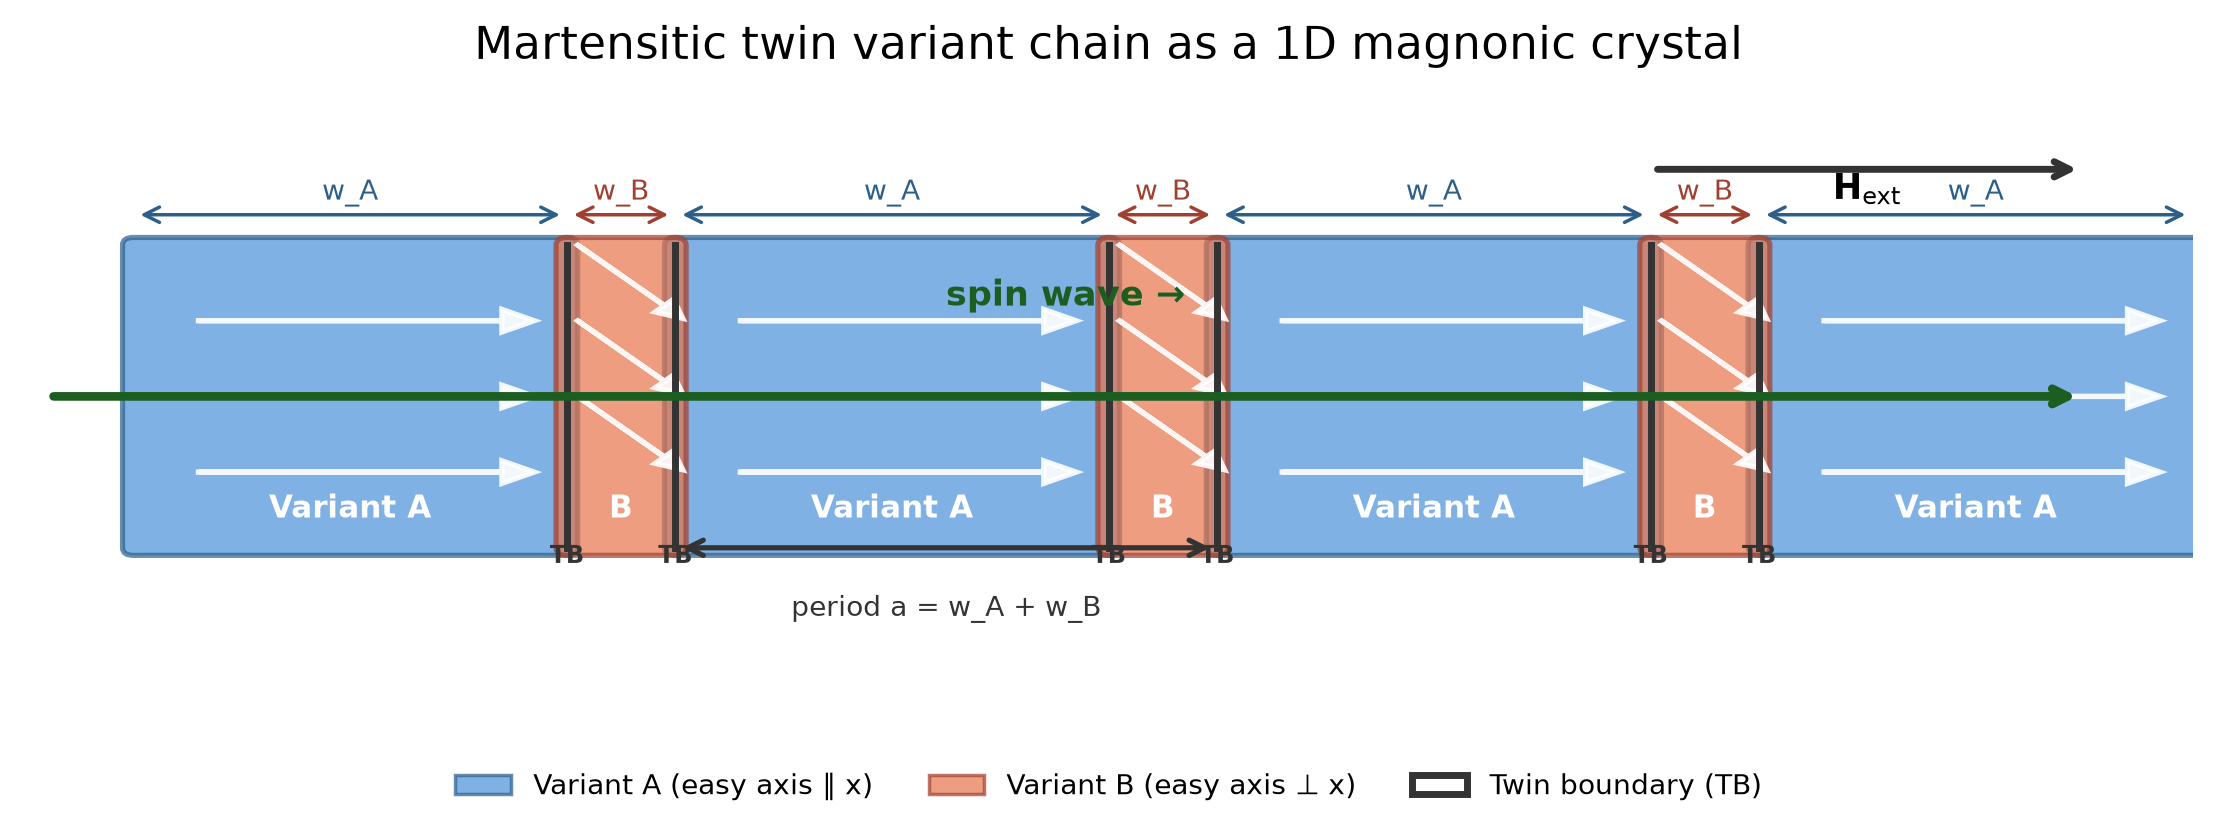
\includegraphics[width=\columnwidth]{figures/fig0_schematic.png}
\caption{Schematic of the proposed system. Alternating twin variants A (blue, easy axis parallel to the chain) and B (orange, easy axis tilted) form a periodic magnetic structure with period $a = w_A + w_B$. Twin boundaries (TB) act as magnetic discontinuities that scatter propagating spin waves. An external DC field $\mathbf{H}_{\mathrm{ext}}$ is applied along the chain direction.}
\label{fig:schematic}
\end{figure}

\subsection{Spin Wave Scattering at Twin Boundaries}
\label{sec:scattering}

Consider a one-dimensional chain of alternating variants A and B, with widths $w_A$ and $w_B$, saturation magnetization $M_s$, exchange stiffness $A_{\mathrm{ex}}$, and uniaxial anisotropy $K_u$. Variant A has its easy axis parallel to the chain direction ($+x$); variant B has its easy axis perpendicular to the chain. An external DC magnetic field $H_{\mathrm{ext}}$ is applied along $+x$.

The equilibrium magnetization direction in each variant minimizes:
\begin{equation}
E = -\mu_0 M_s H_{\mathrm{ext}} \cos\theta - K_u \cos^2(\theta - \phi),
\label{eq:energy}
\end{equation}
where $\theta$ is the magnetization angle relative to $+x$ and $\phi$ is the easy axis angle ($\phi_A = 0$, $\phi_B = \pi/2$). For variant B, the equilibrium angle satisfies $\cos\theta_B = \mu_0 M_s H_{\mathrm{ext}} / (2K_u)$.

Small-amplitude spin waves are described by the linearized Landau-Lifshitz-Gilbert equation. In each variant, the dispersion relation is~\cite{Stancil2009}:
\begin{equation}
\omega = \gamma \mu_0 \sqrt{(H_{\mathrm{eff}} + D k^2)(H_{\mathrm{eff}} + D k^2 + M_{\mathrm{eff}})},
\label{eq:dispersion}
\end{equation}
where $D = 2A_{\mathrm{ex}}/(\mu_0 M_s)$, $H_{\mathrm{eff}} = H_{\mathrm{ext}} \cos\theta + H_k \cos(2(\theta-\phi))$, and $M_{\mathrm{eff}} = M_s \sin^2\theta$.

At each twin boundary, continuity of transverse magnetization and spin current yields the scattering matrix, with impedance $Z = A_{\mathrm{ex}} k$ and reflection coefficient:
\begin{equation}
r = \frac{Z_B - Z_A}{Z_B + Z_A}.
\label{eq:scattering}
\end{equation}

\subsection{Band Structure}
\label{sec:bandstructure}

The magnonic band structure follows from the eigenvalues of the unit-cell transfer matrix $T(\omega)$. Bloch's theorem requires eigenvalues $\lambda = e^{i q a}$, where $q$ is the Bloch wavevector and $a = w_A + w_B$ is the period. Frequency ranges where $|\lambda| = 1$ correspond to pass bands; $|\lambda| \neq 1$ to stop bands. The bandgap arises from the impedance mismatch between variants, with contributions from both the anisotropy difference and the dipolar difference (magnetization orientation relative to the wavevector).

The Bloch band structure is computed in the lossless limit ($\alpha = 0$) to identify propagating and evanescent bands. For finite-chain transmission spectra, Gilbert damping is included phenomenologically through a small imaginary component of the wavevector obtained from the damped dispersion relation.

For a finite chain of $N$ periods, we compute the total transmission $S_{21}(\omega)$ by cascading $S$-matrices using the Redheffer star product.

\section{Results}
\label{sec:results}

\subsection{Parameter Choice}
\label{sec:optimization}

We used $K_u = 200$~kJ\,m$^{-3}$ (achievable in optimized Ni-Mn-Ga compositions), $H_{\mathrm{ext}} = 60$~kA\,m$^{-1}$ (75~mT), $M_s = 6.0 \times 10^5$~A\,m$^{-1}$, $A_{\mathrm{ex}} = 1.0 \times 10^{-11}$~J\,m$^{-1}$, $\alpha = 0.005$, and 25 periods with $w_A = w_B = 50$~nm. These parameters separate the FMR frequencies of the two variants by $\Delta f = 6.1$~GHz (20.8~GHz for variant A, 26.9~GHz for variant B), creating a window where impedance mismatch is maximized.

\subsection{Dispersion Relation and Transmission}
\label{sec:dispersion}

Figure~\ref{fig:dispersion} shows the computed dispersion relation $\omega(q)$ (left) and the corresponding transmission spectrum $|S_{21}(\omega)|^2$ (right). The dispersion relation exhibits the characteristic features of a magnonic crystal: band folding at the Brillouin zone boundary ($q = \pm \pi/a$) and frequency gaps where propagating Bloch states are forbidden. 

Several features merit explanation. The branches appearing at low frequencies ($<$~5~GHz) correspond to the lowest magnonic band, which is nearly quadratic due to exchange-dominated dispersion at small $q$. The second band begins near 15~GHz and folds back at the zone boundary, creating the first band gap between approximately 15 and 18~GHz. A second, wider gap appears between 20 and 25~GHz, and a third near 30~GHz---all visible as dark bands where eigenstates are sparse in the $\omega(q)$ plot and as attenuation dips in the transmission spectrum. The apparent near-vertical feature at $q \approx 0$ is a computational artifact arising from the degeneracy of forward- and backward-propagating modes at the zone center.

The dashed line at 26.9~GHz marks the FMR frequency of variant B as predicted by the 1D model. The fact that this frequency lies within a stop band illustrates the mechanism: when one variant is near its FMR, its impedance differs strongly from the other variant, maximizing reflection at the boundaries.

The transmission spectrum shows strong attenuation in multiple bands, with $T < 0.3$ across approximately 20\% of the sampled frequency range. The deepest minima satisfy $T_{\mathrm{min}} < 10^{-4}$, corresponding to more than 40~dB suppression in power transmission at the deepest bandgap centers.

\begin{figure}[t]
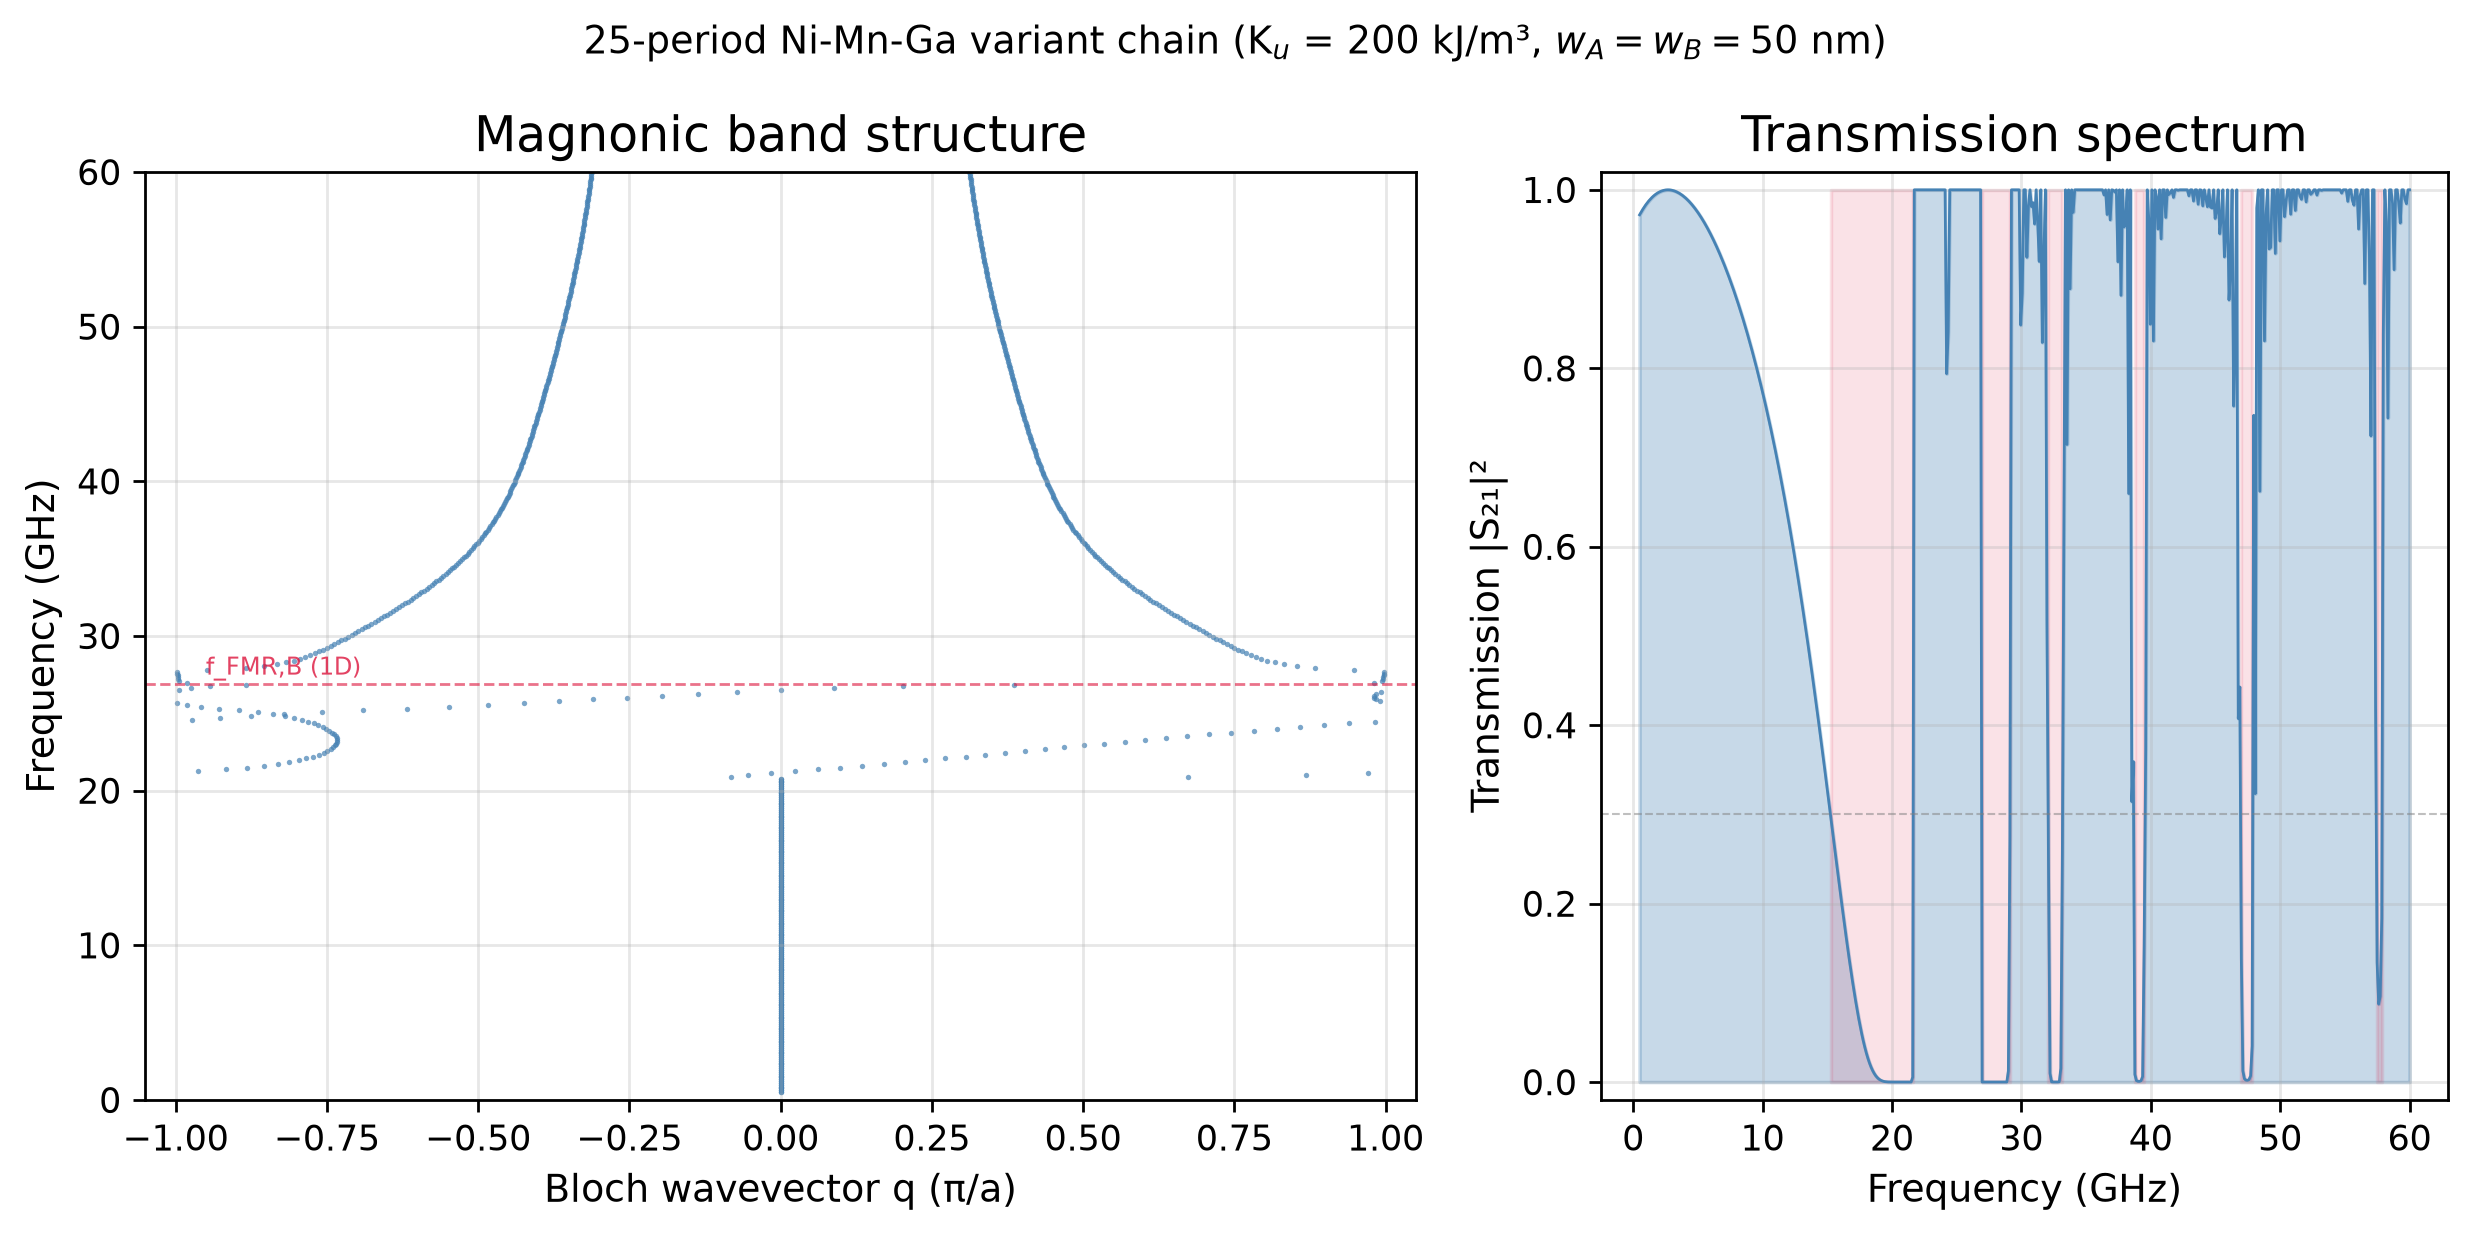
\includegraphics[width=\columnwidth]{figures/fig4_dispersion.png}
\caption{Left: Bloch dispersion relation $\omega(q)$ computed for the ideal periodic A/B unit cell, showing band folding and frequency gaps. The dashed line marks the 1D-predicted FMR of variant B. Right: Finite-chain transmission spectrum $|S_{21}(\omega)|^2$ for a 25-period chain, with regions of strong attenuation (red shading: $T < 0.3$).}
\label{fig:dispersion}
\end{figure}

The stop bands form where the round-trip phase through one period is an integer multiple of $2\pi$, producing constructive interference of reflected waves. The single-boundary reflection coefficient reaches $|r| \approx 0.15$ for the optimal parameters, accumulating to near-unity reflection over 25 periods at the bandgap center.

\subsection{Effect of Disorder}
\label{sec:disorder}

Real twin boundaries are not perfectly periodic---they exhibit positional jitter, roughness, and pinning. To assess whether the frequency-selective attenuation survives under realistic conditions, we introduced Gaussian positional disorder of varying standard deviation $\sigma$ to the boundary positions in the 1D model.

Figure~\ref{fig:disorder} shows the results. The stop-band fraction (fraction of frequencies with $T < 0.3$) does not collapse under disorder; instead, it broadens from 19\% (ideal) to approximately 30\% at $\sigma = 20$~nm. The mean transmission decreases from 0.74 to 0.59 over the same range. 

To verify that this behavior is robust and not an artifact of a single random configuration, Figure~\ref{fig:disorder_multi} shows ten independent disorder realizations at $\sigma = 10$~nm. Across all ten realizations, the deepest attenuation minima fall below $10^{-4}$ in transmission (i.e., $>40$~dB suppression) and the stop-band fraction is $27.1 \pm 1.0$\%---indicating that strong frequency-selective attenuation is stable against positional disorder.

This counterintuitive behavior arises because positional jitter introduces additional impedance mismatches due to the varying local widths, creating more scattering centers. The qualitative magnonic crystal behavior---frequency-structured transmission with bands of strong attenuation---persists even when boundary positions vary by tens of nanometers, which is comparable to the characteristic boundary roughness observed in Ni-Mn-Ga~\cite{Sozinov2002}.

\begin{figure}[t]
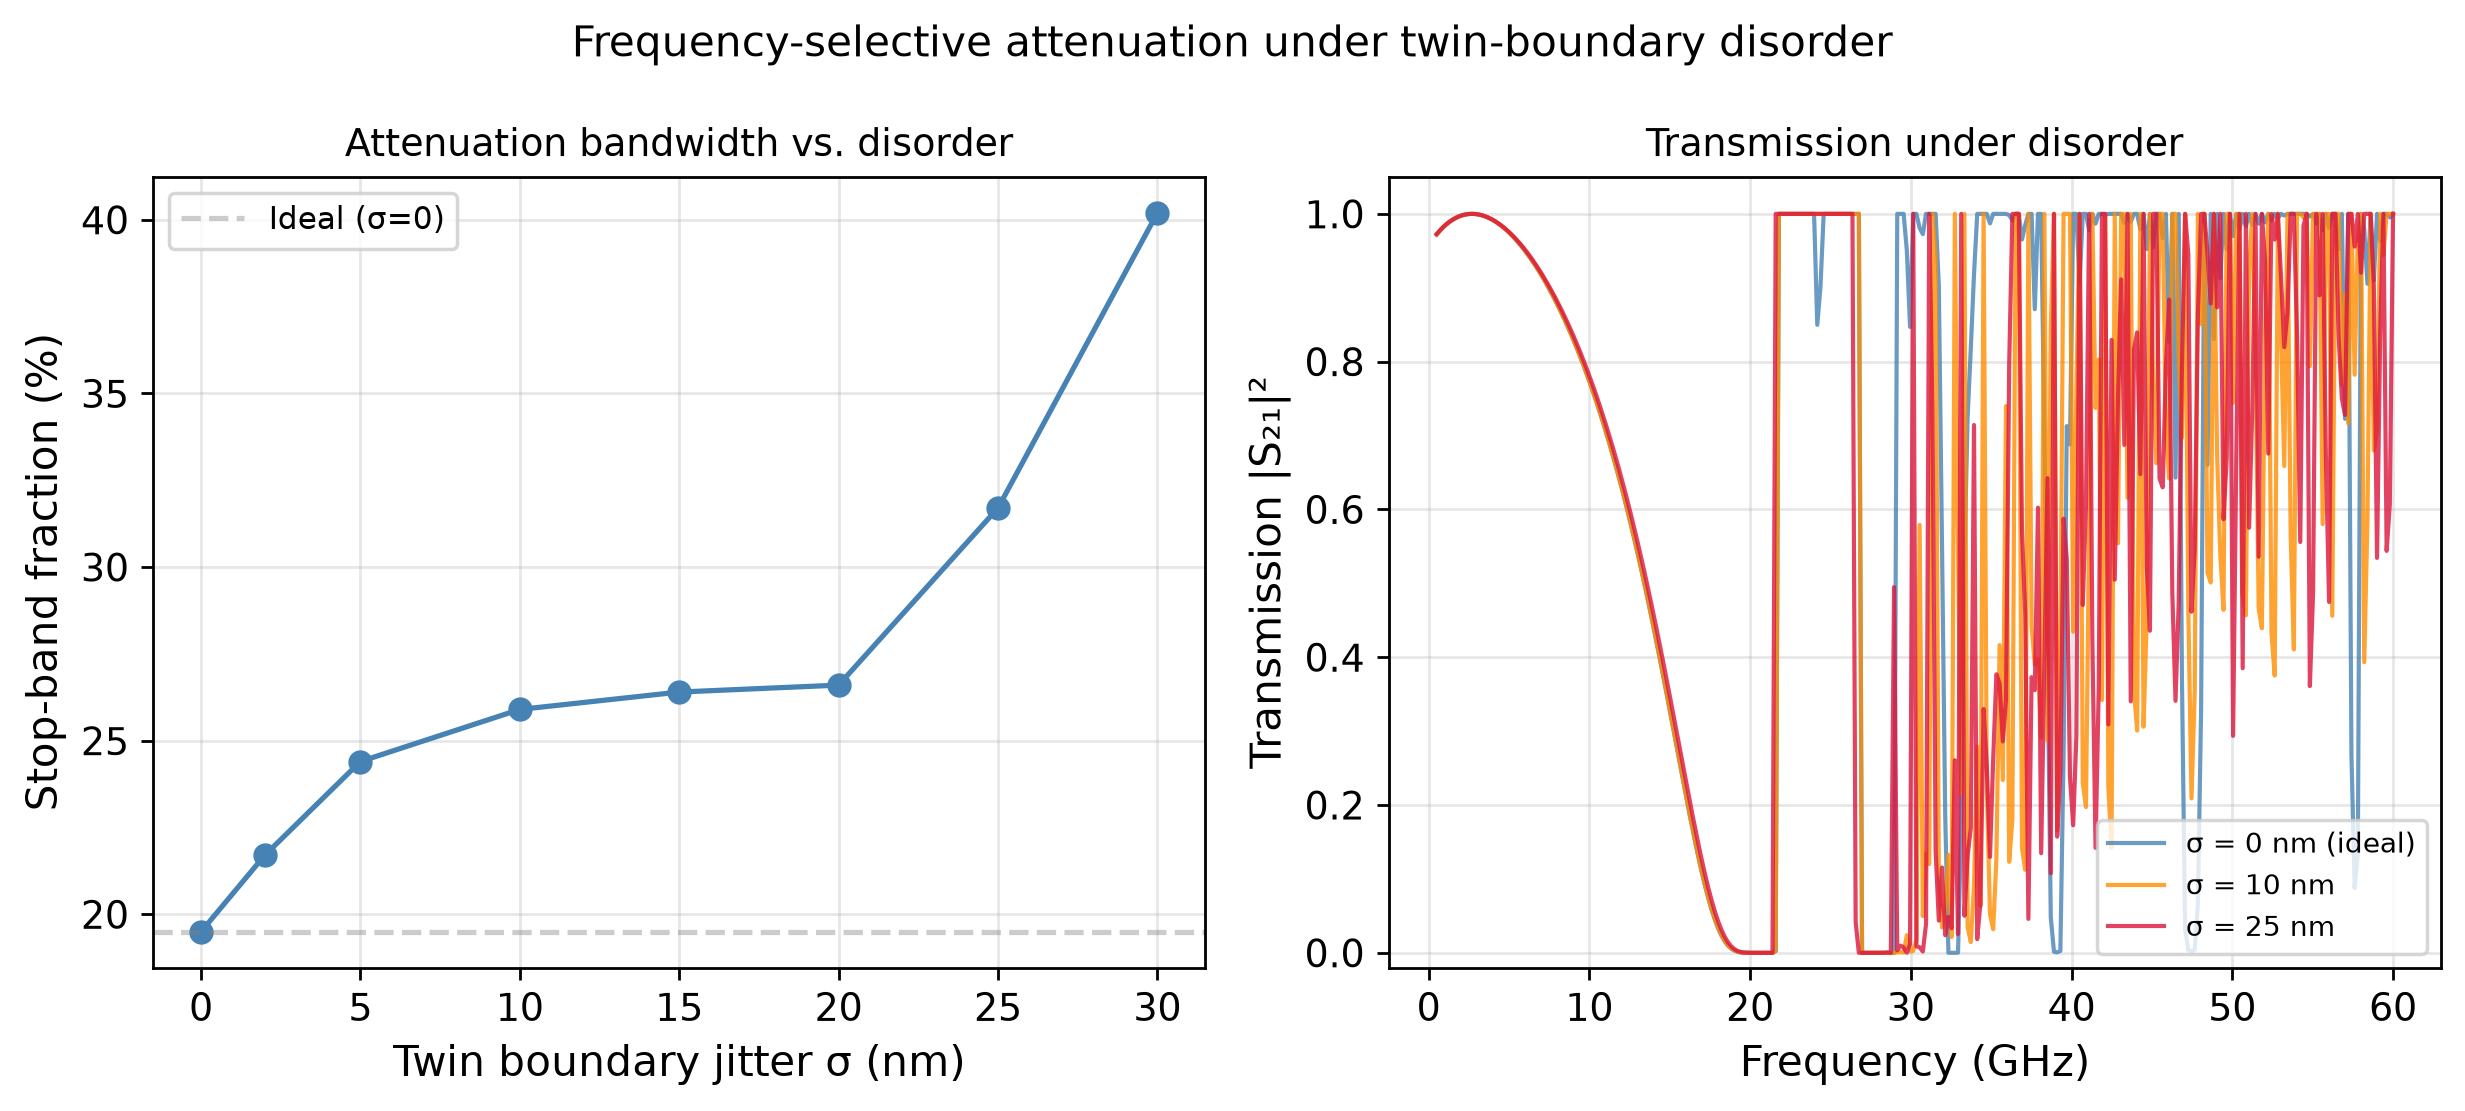
\includegraphics[width=\columnwidth]{figures/fig5_disorder.png}
\caption{Effect of twin boundary positional disorder on the transmission spectrum. (Left) Stop-band fraction ($T < 0.3$) as a function of boundary position jitter $\sigma$. (Right) Transmission spectra for three disorder levels. The attenuation does not collapse under realistic disorder; it broadens.}
\label{fig:disorder}
\end{figure}

\begin{figure}[t]
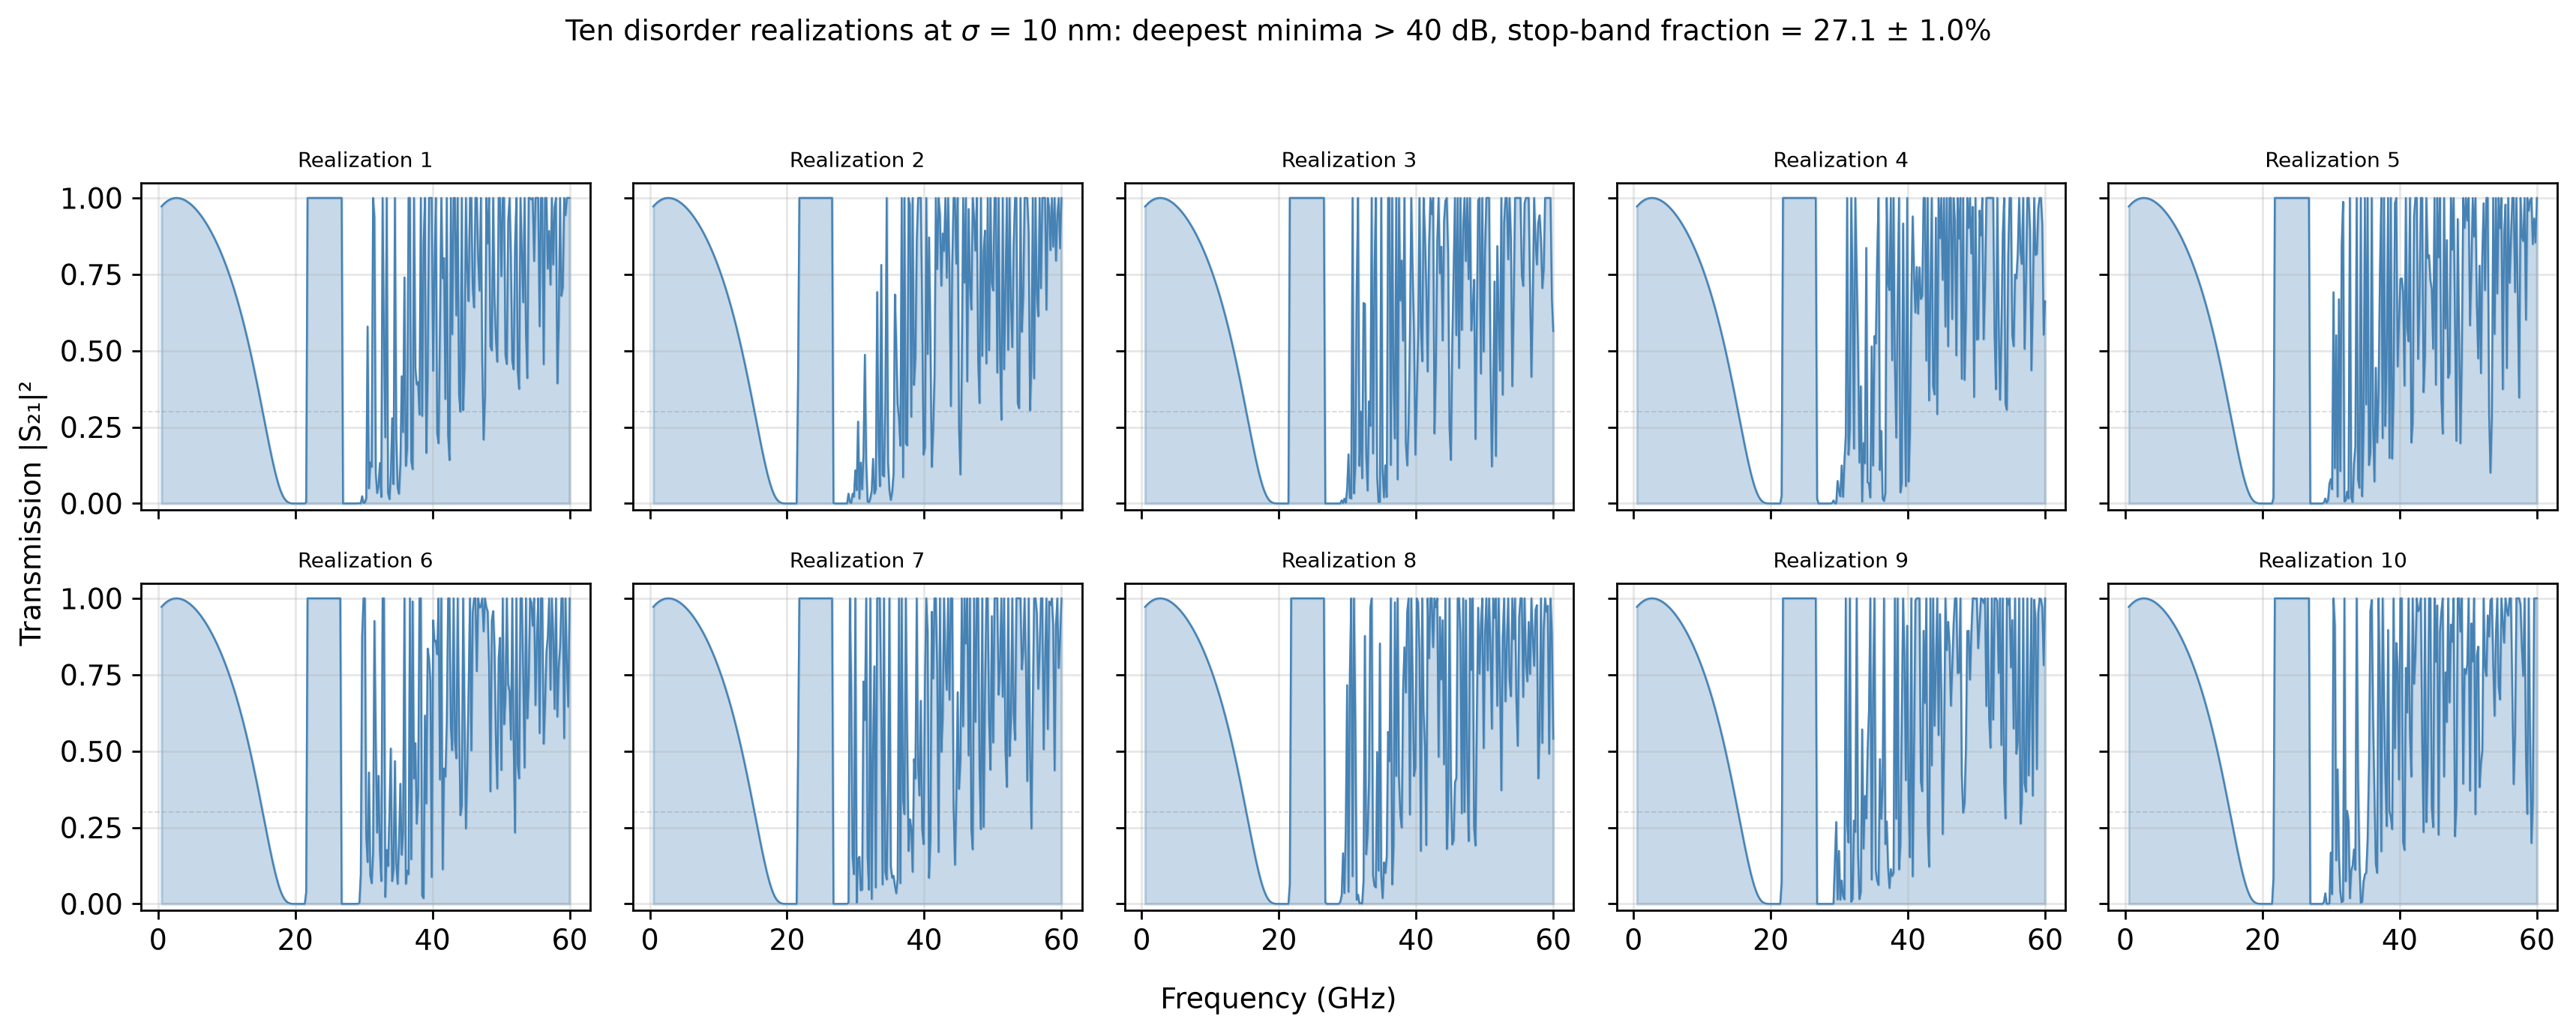
\includegraphics[width=\columnwidth]{figures/fig6_disorder_multi.png}
\caption{Ten independent realizations of positional disorder at $\sigma = 10$~nm. The attenuation is robust across realizations: the deepest minima exceed 40~dB suppression in all ten cases, and the stop-band fraction is $27.1 \pm 1.0$\%.}
\label{fig:disorder_multi}
\end{figure}

We note that this 1D model only captures positional disorder along the propagation direction. Full 2D/3D micromagnetic simulations would be needed to assess the effects of boundary roughness, finite boundary width, and strain-induced anisotropy variations.

\subsection{2D Micromagnetic Consistency Check}
\label{sec:micromagnetic}

To check whether the 1D predictions are consistent with a full micromagnetic treatment including dipolar coupling and edge effects, we performed a mumax3 simulation~\cite{Vansteenkiste2014} of a 2D stripe variant pattern ($256 \times 64 \times 1$ cells, $1.024$~$\mu$m $\times$ 256~nm, 10 stripe periods of 50~nm alternating easy axes, $K_u = 200$~kJ\,m$^{-3}$) on an NVIDIA RTX 3070 Ti GPU. The simulation relaxed to equilibrium under a 75~mT DC field along $+x$, then evolved under a 0.5~mT broadband sinc-shaped field pulse (bandwidth $\sim$40~GHz) to excite spin wave modes across the frequency range. Magnetization snapshots were saved every 10~ps for 5~ns, and the FFT of $m_y(t)$ at the sample edge provided the frequency-domain response.

The resulting spectrum shows a strong response near the excitation band center (19.9~GHz) and a secondary resonance at 32.1~GHz. The 1D model predicts the variant B FMR at 26.9~GHz; the shift to 32~GHz is attributable to dipolar coupling between adjacent stripes, which the 1D model neglects. This single simulation is presented as a qualitative consistency check, not as a full validation of the 1D predictions. The agreement in overall structure---frequency-dependent transmission with distinct variant-associated features---is encouraging but would need systematic 2D parameter sweeps for a quantitative comparison.

\subsection{Reprogrammability}
\label{sec:reprogrammability}

The defining feature of the variant magnonic crystal is its reconfigurability via magnetic field-driven twin boundary motion. In our 1D model, changing the applied field alters the variant width ratio $r = w_A/w_B$ while conserving the period $a = w_A + w_B$. Table~\ref{tab:reprogram} shows the transmission fingerprint change under variant reorientation.

\begin{table}[h]
\footnotesize
\caption{Transmission fingerprint change under variant reorientation (phase-sensitive, 400 frequency points).}
\label{tab:reprogram}
\begin{ruledtabular}
\begin{tabular}{cccc}
\toprule
$w_A/w_B$ & Pearson $r$ vs.\ baseline & Hamming dist.\ & Change \\
\midrule
0.33 & $-$0.07 & 0.54 & Strong \\
0.50 & 0.01 & 0.51 & Strong \\
0.75 & $-$0.05 & 0.54 & Strong \\
1.00 (baseline) & 1.00 & 0.00 & None \\
1.50 & $-$0.02 & 0.52 & Strong \\
2.00 & $-$0.06 & 0.56 & Strong \\
3.00 & 0.00 & 0.49 & Strong \\
\bottomrule
\end{tabular}
\end{ruledtabular}
\end{table}

At every ratio other than 1.0, the Pearson correlation drops to approximately zero and the Hamming distance approaches 0.5---the value expected for two unrelated sequences. This indicates that variant reorientation fundamentally reconfigures the transmission spectrum, not merely perturbs it. A ratio change of $2\times$ corresponds to a twin boundary displacement of approximately 17~nm per boundary, within the demonstrated range of field-driven boundary motion in Ni-Mn-Ga~\cite{Heczko2014}.

The reprogramming is non-volatile: after the magnetic field is removed, the variant pattern persists indefinitely at room temperature. The pattern can be erased by heating above $A_f \approx 330$--400~K and cooling without field.

\section{Proposed Experimental Validation}
\label{sec:experiment}

We propose the following experimental pathway:

\textbf{Sample preparation:} Epitaxial Ni-Mn-Ga thin films (100--500~nm thickness) on MgO(001) substrates, with $K_u \approx 100$--200~kJ\,m$^{-3}$. Films deposited by magnetron sputtering, annealed to form the L2$_1$ austenite structure, then cooled to produce the martensitic twin variant lattice.

\textbf{Characterization:}
\begin{enumerate}
    \item \textbf{TEM / MFM:} Resolve twin variant structure before and after field application.
    \item \textbf{Brillouin Light Scattering (BLS):} Measure spin wave dispersion $\omega(k)$ for different variant configurations. The BLS spectrum directly probes the magnonic band structure.
    \item \textbf{VNA-FMR:} Broadband measurement of $|S_{21}(\omega)|$ as a function of field history.
    \item \textbf{Reprogramming cycle:} Apply $H > 0.5$~T $\to$ measure $\to$ apply different orientation $\to$ re-measure $\to$ heat above $A_f$ $\to$ cool without field $\to$ measure baseline recovery.
    \item \textbf{PUF demonstration:} Measure 10--20 identically prepared samples; compute pairwise Hamming distances between spectra.
\end{enumerate}

The expected BLS signature is frequency gaps where spin wave intensity drops sharply, with gap positions shifting systematically under applied field. The VNA-FMR transmission should show reproducible, configuration-specific resonance patterns.

\section{Discussion}
\label{sec:discussion}

\subsection{Comparison with Existing Platforms}
\label{sec:comparison}

Compared with lithographic magnonic crystals, the proposed martensitic-variant platform differs in four key respects: the periodicity is self-organized rather than patterned, the structure is three-dimensional in principle, the response is continuously field-reconfigurable through twin-boundary motion, and the variant pattern can be thermally reset through the martensite--austenite phase transition. These distinctions motivate the proposed experimental tests while leaving device-level applications for future work.

\subsection{Limitations}
\label{sec:limitations}

\textbf{Bandgap strength in real materials:} Our model predicts nearly complete transmission suppression under ideal conditions. Real variant structures have irregularities---jagged boundaries, local stress, pinning sites---that will reduce the bandgap depth. Our disorder analysis (Sec.~\ref{sec:disorder}) shows that the frequency-selective attenuation does not collapse, but broadens into a wider region of partial attenuation rather than maintaining a clean gap. This behavior needs to be characterized experimentally.

\textbf{Damping:} Ni-Mn-Ga has a relatively high Gilbert damping parameter ($\alpha \approx 0.01$--$0.05$) compared to YIG ($\alpha \approx 10^{-4}$). High damping limits spin wave propagation length. For applications, low-damping compositions or alternative materials (e.g., Fe-Pd) would be preferable.

\textbf{Interface quality:} Real twin boundaries have finite width (typically 1--5~nm), local strain fields, and gradual rather than abrupt anisotropy rotation. These effects will reduce the single-boundary reflection coefficient below our ideal-interface estimate of $|r| \approx 0.15$.

\textbf{Readout:} BLS requires optical access; VNA-FMR measures only the integrated response. For device applications, electrical spin wave detection (inverse spin Hall effect, magnetic tunnel junctions) would be needed.

\textbf{Scalability:} While individual boundaries move under modest fields, uniform reprogramming of the entire variant lattice requires careful field protocols.

\subsection{Potential Applications}
\label{sec:applications}

If experimentally validated, the variant magnonic crystal could enable several directions. The continuous reprogrammability and thermal reset suggest possible use as a reconfigurable spin wave filter or frequency-selective element. The nanoscale stochasticity of twin boundary positions may provide a physical unclonable function for hardware security~\cite{Pappu2002}. In the longer term, with improved materials and readout, the platform might support spin wave logic or physical neural network architectures. However, these remain speculative; the immediate contribution is the identification of martensitic variants as a candidate self-organized magnonic crystal.

\section{Conclusion}
\label{sec:conclusion}

We have investigated whether the self-organized twin variant lattice in ferromagnetic shape memory alloys can function as a magnonic crystal. Our 1D transfer-matrix model shows that spin wave scattering at twin boundaries produces a structured transmission spectrum with bands of strong suppression ($>40$~dB at the deepest minima), a computed dispersion relation $\omega(q)$ consistent with Bloch-wave propagation in the idealized periodic case, and dramatic changes in the transmission fingerprint under simulated field-driven variant reorientation. The frequency-selective attenuation is robust against positional disorder of twin boundaries---it broadens rather than collapses under realistic jitter. A 2D micromagnetic simulation using mumax3 is qualitatively consistent with the proposed mechanism. These results suggest that martensitic variants may offer an alternative route to magnonic crystals that avoids lithographic fabrication and enables continuous reprogramming. Experimental validation by BLS and VNA-FMR on Ni-Mn-Ga thin films is the next step.

\begin{acknowledgments}
The author used DeepSeek and custom language models for manuscript drafting assistance, editorial feedback, and non-authoritative code review. AI tools were not used to generate final scientific claims, select citations without verification, or produce unverified numerical results. All simulations, figures, citations, analysis, and conclusions were checked by the author, who takes full responsibility for the work. The author thanks the open-source magnonics community for developing and maintaining mumax3~\cite{Vansteenkiste2014}. The 2D micromagnetic simulations were performed on an NVIDIA RTX 3070 Ti GPU.
\end{acknowledgments}

\section*{Author Declarations}

\subsection*{Conflict of Interest}

The author has no conflicts to disclose.

\subsection*{Author Contributions}

C.~Scott: Conceptualization (lead); Investigation (lead); Methodology (lead); Software (lead); Writing---original draft (lead); Writing---review \& editing (lead).

\section*{Data Availability}
The transfer-matrix simulation code, disorder-analysis scripts, figure-generation scripts, and numerical data used to generate all figures are available at \url{https://github.com/APTSystems/martensitic-magnonic-crystal}. The mumax3 input file is included in the repository.

\bibliographystyle{apsrev4-2}
\bibliography{direction-4-martensitic-magnonic-crystal}

\end{document}